\paragraph{La classe SendFrames}

\begin{minipage}
    {\linewidth}
    \centering
    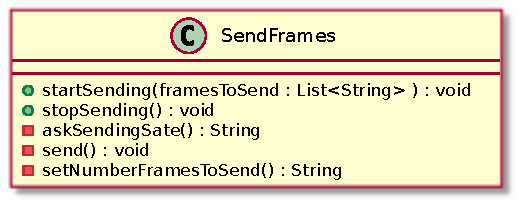
\includegraphics[width=\linewidth]{../schemas/Conception_detaillee/diag_class_sender_client.pdf}
    \captionof{figure}{Diagramme de classe de SendFrames}
\end{minipage}

\subparagraph{Philosophie de conception \newline} 

\medspace

La classe SendFrames a pour rôle d'envoyer les trames au programme {\nomLogiciel}.  

\subparagraph{Description structurelle \newline}

\medspace

\textbf{Attributs :}

N.A.

\textbf{Services offerts :}

\begin{itemize}
    \item \textbf{startSending(framesToSend : List<String>) : void} --- Opération qui permet de commencer à envoyer des trames. 
    \item \textbf{stopSending() : void } --- Opération qui permet d'arrêter l'envoi des trames. 
    \item \textbf{askSendingState() : String } --- Opération qui permet l'envoi de la demande d'état afin de savoir si les trames sont en cours d'envoi ou non. 
    \item \textbf{send() : void} --- Opération qui envoie les différentes informations à envoyer ainsi que les trames. 
    \item \textbf{setNumberFramesToSend() : String } --- Opération qui permet de connaitre le nombre de trames à envoyer et retourne le nombre sous la forme "nb=X" où X est le nombre de trames à envoyer. 
\end{itemize}